\documentclass{beamer}
\usepackage{amsmath,amsbsy,amsopn,amstext,amsfonts,amssymb}
\usepackage{isomath}
\usepackage{ulem}
%\linespread{1.6}  % double spaces lines
\usepackage{graphicx}
\usepackage{subfigure}
\usepackage{color}
\usepackage{optidef}  % define optimization problems
\usepackage{multicol}  % multiple columns
\usepackage{listings} % for python code
\usepackage{mathrsfs}

\usepackage{polynom}
\newcommand{\adj}{\mathrm{adj}}
\newcommand{\constrainedmin}[3]{
		\begin{mini*}|s|
		{#2}{#1}{}{}
		\addConstraint{#3}
		\end{mini*}
}

\newcommand{\rwbcomment}[1]{{\color{blue}RWB:#1}}
\newcommand{\defeq}{\stackrel{\triangle}{=}}
\newcommand{\abs}[1]{\left|#1\right|}
\newcommand{\norm}[1]{\left\|#1\right\|}
\newcommand{\iprod}[1]{\left<#1\right>}
\newcommand{\ellbf}{\boldsymbol{\ell}}
\newcommand{\nubf}{\boldsymbol{\nu}}
\newcommand{\mubf}{\boldsymbol{\mu}}
\newcommand{\abf}{\mathbf{a}}
\newcommand{\bbf}{\mathbf{b}}
\newcommand{\cbf}{\mathbf{c}}
\newcommand{\dbf}{\mathbf{d}}
\newcommand{\ebf}{\mathbf{e}}
\newcommand{\fbf}{\mathbf{f}}
\newcommand{\gbf}{\mathbf{g}}
\newcommand{\hbf}{\mathbf{h}}
\newcommand{\ibf}{\mathbf{i}}
\newcommand{\jbf}{\mathbf{j}}
\newcommand{\kbf}{\mathbf{k}}
\newcommand{\lbf}{\mathbf{l}}
\newcommand{\mbf}{\mathbf{m}}
\newcommand{\nbf}{\mathbf{n}}
\newcommand{\obf}{\mathbf{o}}
\newcommand{\pbf}{\mathbf{p}}
\newcommand{\qbf}{\mathbf{q}}
\newcommand{\rbf}{\mathbf{r}}
\newcommand{\sbf}{\mathbf{s}}
\newcommand{\tbf}{\mathbf{t}}
\newcommand{\ubf}{\mathbf{u}}
\newcommand{\vbf}{\mathbf{v}}
\newcommand{\wbf}{\mathbf{w}}
\newcommand{\xbf}{\mathbf{x}}
\newcommand{\ybf}{\mathbf{y}}
\newcommand{\zbf}{\mathbf{z}}
\newcommand{\Jbf}{\mathbf{J}}
\newcommand{\Acal}{\mathcal{A}}
\newcommand{\Bcal}{\mathcal{B}}
\newcommand{\Lcal}{\mathcal{L}}
\newcommand{\Ncal}{\mathcal{N}}
\newcommand{\Rcal}{\mathcal{R}}
\definecolor{darkolivegreen}{rgb}{0.33, 0.42, 0.18}

\makeatletter
\newenvironment<>{proofstart}[1][\proofname]{%
    \par
    \def\insertproofname{#1\@addpunct{.}}%
    \usebeamertemplate{proof begin}#2}
  {\usebeamertemplate{proof end}}
\newenvironment<>{proofcont}{%
  \setbeamertemplate{proof begin}{\begin{block}{}}
    \par
    \usebeamertemplate{proof begin}}
  {\usebeamertemplate{proof end}}
\newenvironment<>{proofend}{%
    \par
    \pushQED{\qed}
    \setbeamertemplate{proof begin}{\begin{block}{}}
    \usebeamertemplate{proof begin}}
  {\popQED\usebeamertemplate{proof end}}
\makeatother

\title{ECEn 671: Mathematics of Signals and Systems}
\author{Randal W. Beard}
\institute{Brigham Young University}
\date{\today}

\begin{document}

%-------------------------------
\begin{frame}
	\titlepage
\end{frame}




%%%%%%%%%%%%%%%%%%%%%%%%%%%%%%%%%%%%%%%%%%%%%%%%%%%%%%%%%%%%%%%%%
\section{Adjoint Operators}
\frame{\sectionpage}

%----------------------------------
\begin{frame}\frametitle{Adjoint Operator}
	\begin{definition}
		Let $\Acal: \mathbb{X} \to \mathbb{Y}$ be a bounded linear operator from Hilbert space $\mathbb{X}$ to Hilbert space $\mathbb{Y}$, then the \underline{adjoint of $\Acal$} ($\Acal^\ast$) is the linear operator $\Acal^\ast:\mathbb{Y}\to\mathbb{X}$ such that
			\[ 
			\iprod{\Acal x,y }_{\mathbb{Y}} = \iprod{x,\Acal^\ast y }_{\mathbb{X}} 
			\]
			$\forall x\in\mathbb{X}$ and $\forall y \in \mathbb{Y}$.  
			
			\vspace{1cm}
			
			$\Acal$ is \underline{self-adjoint} if $\Acal^\ast=\Acal$
	\end{definition}
\end{frame}

%----------------------------------
\begin{frame}\frametitle{Adjoint Operator, Example}
	\begin{example}[Complex matrices]
		$A:\mathbb{C}^n \to \mathbb{C}^m$	
			
		\vspace{0.5cm}
		What is $A^\ast$?
		\vspace{0.5cm}
		
		By definition:
		\begin{align*}
			& 	\iprod{Ax,y }_{\mathbb{C}^m} = \iprod{x,A^\ast y }_{\mathbb{C}^n} \\
			\iff & y^HAx = y^H (A^\ast)^H x \\
			\iff & A^\ast = A^H
		\end{align*}
		\vspace{0.5cm}
		Note $A^H : \mathbb{C}^m \to \mathbb{C}^n$
	\end{example}
\end{frame}


%----------------------------------
\begin{frame}\frametitle{Adjoint Operator, Example}
	\begin{example}[Real matrices]
		$A:\mathbb{R}^n \to \mathbb{R}^m$
		
		\vspace{0.5cm}
		What is $A^\ast$?
		\vspace{0.5cm}
		
		By definiton, 
			\begin{align*}
				& \iprod{Ax,y }_{\mathbb{R}^m} = \iprod{x,A^\ast y }_{\mathbb{R}^n} \\
				\iff & x^\top A^\top y = x^\top A^\ast y \\
				\iff & A^\ast = A^\top
			\end{align*}
	\end{example}
\end{frame}

%----------------------------------
\begin{frame}\frametitle{Adjoint Operator, Example}
	\begin{example}[Convolution]
		\[ \Acal:L_2 \to L_2 \]
		\[ \Acal[x](t) = \int_{0}^\top h(t-\tau) x(\tau) d\tau \]
		Let $x \in L_2[0,\infty]$ and $y \in L_2[0,\infty]$ then $\Acal^\ast$ is defined by
		\[ \iprod{\Acal x,y }_{L_2} = \iprod{x,\Acal^\ast y }_{L_2} 
		\]
		\[ \iff \int_{t=0}^{\infty} \left[ \int_{\tau = 0}^t h(t-\tau)x(\tau)d\tau \right] y(t) dt = \int_0^{\infty}x(t)\Acal^\ast[y](t)dt \]
	\end{example}
\end{frame}

%----------------------------------
\begin{frame}\frametitle{Adjoint Operator, Example, Convolution, cont.}
	\begin{center}
	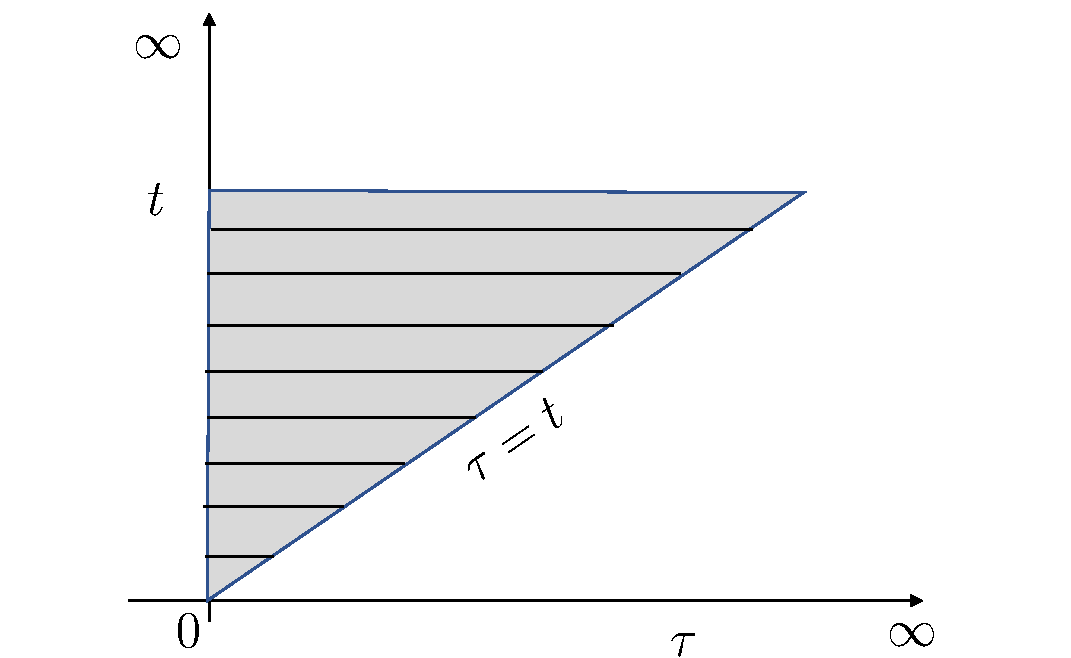
\includegraphics{figures/chap4_order_of_integration}
	\end{center}

	Change the order of integration to get
	\begin{align*}
	\int_{\tau=0}^{\infty} \int_{t=\tau}^{\infty} h(t-\tau)x(\tau)y(t)dt d\tau &= \int_0^{\infty} x(t) \int_t^{\infty} h(\tau - t) y(\tau) d\tau dt\\
	&= \int_0^{\infty} x(t)A^\ast[y](t)dt
	\end{align*}
	\[ \Rightarrow \Acal^\ast[y] = \int_t^{\infty}h(\tau - t)y(\tau)d\tau \]
\end{frame}

%----------------------------------
\begin{frame}\frametitle{Adjoint Operator, Example}
	\begin{example}[linear ode's]
		\[ \dot{x} = Fx \quad ; \quad x(0) = x_0 \]
		
		\vfill
		
		The solution is $x(t) = e^{Ft}x_0$
		
		\vfill
		
		Let $\Acal[x_0](t) = e^{Ft}x_0$, then
		\[ \Acal:\mathbb{R}^n \to L_{2[0,T]} \]
		
		\vfill 
		
		What is $\Acal^\ast$?
	\end{example}
\end{frame}

%----------------------------------
\begin{frame}\frametitle{Adjoint Operator, Example, linear ODE, cont.}
	Let $x \in \mathbb{R}^n$ and let $y \in L_2[0,T]$ then by definition,
		\begin{align*}
			\iprod{\Acal[x_0],y }_{L_2[0,T]} &= \iprod{x_0, \Acal^\ast y }_{\mathbb{R}^n} \\
			\iff \int_0^T x_0^\top(e^{Ft})^\top y(t)dt &= x_0^\top \Acal^\ast y \\
			\iff x_0^\top \int_0^T e^{F^\top t}y(t) dt &= x_0^\top \Acal^\ast y \\
			\Rightarrow \fbox{ $\Acal^\ast[y] = \displaystyle \int_0^Te^{F^\top t}y(t)dt $ }\\
		\end{align*}
\end{frame}




\end{document}